\documentclass[journal,12pt,twocolumn]{IEEEtran}
\makeatletter
\@addtoreset{figure}{problem}
\makeatother
\usepackage{setspace}
\usepackage{gensymb}
\usepackage{xcolor}
\usepackage{caption}
%\usepackage{multirow}
%\usepackage{multicolumn}
%\usepackage{subcaption}
%\doublespacing
\singlespacing
\usepackage{amsmath}
\usepackage{multicol}
\usepackage{enumerate}
\usepackage{amssymb}
\usepackage{graphicx}
\usepackage{newfloat}
%\usepackage{syntax}
\usepackage{listings}
\usepackage{color}
\usepackage{tikz}
\usetikzlibrary{shapes,arrows}



%\usepackage{graphicx}
%\usepackage{amssymb}
%\usepackage{relsize}
%\usepackage[cmex10]{amsmath}
%\usepackage{mathtools}
%\usepackage{amsthm}
%\interdisplaylinepenalty=2500
%\savesymbol{iint}
%\usepackage{txfonts}
%\restoresymbol{TXF}{iint}
%\usepackage{wasysym}
\usepackage{amsthm}
\usepackage{mathrsfs}
\usepackage{txfonts}
\usepackage{stfloats}
\usepackage{cite}
\usepackage{cases}
\usepackage{mathtools}
\usepackage{caption}
\usepackage{enumerate}	
\usepackage{enumitem}
\usepackage{amsmath}
%\usepackage{xtab}
\usepackage{longtable}
\usepackage{multirow}
%\usepackage{algorithm}
%\usepackage{algpseudocode}
\usepackage{enumitem}
\usepackage{mathtools}
%\usepackage{iithtlc}
%\usepackage[framemethod=tikz]{mdframed}
\usepackage{listings}
\usepackage{listings}
    %\usepackage[latin1]{inputenc}                                 %%
    \usepackage{color}                                            %%
    \usepackage{array}                                            %%
    \usepackage{longtable}                                        %%
    \usepackage{calc}                                             %%
    \usepackage{multirow}                                         %%
    \usepackage{hhline}                                           %%
    \usepackage{ifthen}                                           %%
  %optionally (for landscape tables embedded in another document): %%
    \usepackage{lscape}     



%\usepackage{stmaryrd}


%\usepackage{wasysym}
%\newcounter{MYtempeqncnt}
\DeclareMathOperator*{\Res}{Res}
%\renewcommand{\baselinestretch}{2}
\renewcommand\thesection{\arabic{section}}
\renewcommand\thesubsection{\thesection.\arabic{subsection}}
\renewcommand\thesubsubsection{\thesubsection.\arabic{subsubsection}}

\renewcommand\thesectiondis{\arabic{section}}
\renewcommand\thesubsectiondis{\thesectiondis.\arabic{subsection}}
\renewcommand\thesubsubsectiondis{\thesubsectiondis.\arabic{subsubsection}}

% correct bad hyphenation here
\hyphenation{op-tical net-works semi-conduc-tor}

%\lstset{
%language=C,
%frame=single, 
%breaklines=true
%}

%\lstset{
	%%basicstyle=\small\ttfamily\bfseries,
	%%numberstyle=\small\ttfamily,
	%language=Octave,
	%backgroundcolor=\color{white},
	%%frame=single,
	%%keywordstyle=\bfseries,
	%%breaklines=true,
	%%showstringspaces=false,
	%%xleftmargin=-10mm,
	%%aboveskip=-1mm,
	%%belowskip=0mm
%}

%\surroundwithmdframed[width=\columnwidth]{lstlisting}
\def\inputGnumericTable{}                                 %%
\lstset{
language=C,
frame=single, 
breaklines=true
}
 

\begin{document}
%
\tikzstyle{block} = [rectangle, draw,
    text width=3em, text centered, minimum height=3em]
\tikzstyle{sum} = [draw, circle, node distance=3cm]
\tikzstyle{input} = [coordinate]
\tikzstyle{output} = [coordinate]
\tikzstyle{pinstyle} = [pin edge={to-,thin,black}]

\theoremstyle{definition}
\newtheorem{theorem}{Theorem}[section]
\newtheorem{problem}{Problem}
\newtheorem{proposition}{Proposition}[section]
\newtheorem{lemma}{Lemma}[section]
\newtheorem{corollary}[theorem]{Corollary}
\newtheorem{example}{Example}[section]
\newtheorem{definition}{Definition}[section]
%\newtheorem{algorithm}{Algorithm}[section]
%\newtheorem{cor}{Corollary}
\newcommand{\BEQA}{\begin{eqnarray}}
\newcommand{\EEQA}{\end{eqnarray}}
\newcommand{\define}{\stackrel{\triangle}{=}}

\bibliographystyle{IEEEtran}
%\bibliographystyle{ieeetr}

\providecommand{\nCr}[2]{\,^{#1}C_{#2}} % nCr
\providecommand{\nPr}[2]{\,^{#1}P_{#2}} % nPr
\providecommand{\mbf}{\mathbf}
\providecommand{\pr}[1]{\ensuremath{\Pr\left(#1\right)}}
\providecommand{\qfunc}[1]{\ensuremath{Q\left(#1\right)}}
\providecommand{\sbrak}[1]{\ensuremath{{}\left[#1\right]}}
\providecommand{\lsbrak}[1]{\ensuremath{{}\left[#1\right.}}
\providecommand{\rsbrak}[1]{\ensuremath{{}\left.#1\right]}}
\providecommand{\brak}[1]{\ensuremath{\left(#1\right)}}
\providecommand{\lbrak}[1]{\ensuremath{\left(#1\right.}}
\providecommand{\rbrak}[1]{\ensuremath{\left.#1\right)}}
\providecommand{\cbrak}[1]{\ensuremath{\left\{#1\right\}}}
\providecommand{\lcbrak}[1]{\ensuremath{\left\{#1\right.}}
\providecommand{\rcbrak}[1]{\ensuremath{\left.#1\right\}}}
\theoremstyle{remark}
\newtheorem{rem}{Remark}
\newcommand{\sgn}{\mathop{\mathrm{sgn}}}
\providecommand{\abs}[1]{\left\vert#1\right\vert}
\providecommand{\res}[1]{\Res\displaylimits_{#1}} 
\providecommand{\norm}[1]{\lVert#1\rVert}
\providecommand{\mtx}[1]{\mathbf{#1}}
\providecommand{\mean}[1]{E\left[ #1 \right]}
\providecommand{\fourier}{\overset{\mathcal{F}}{ \rightleftharpoons}}
%\providecommand{\hilbert}{\overset{\mathcal{H}}{ \rightleftharpoons}}
\providecommand{\system}{\overset{\mathcal{H}}{ \longleftrightarrow}}
	%\newcommand{\solution}[2]{\textbf{Solution:}{#1}}
\newcommand{\solution}{\noindent \textbf{Solution: }}
\providecommand{\dec}[2]{\ensuremath{\overset{#1}{\underset{#2}{\gtrless}}}}
\DeclarePairedDelimiter{\ceil}{\lceil}{\rceil}
%\numberwithin{equation}{subsection}
\numberwithin{equation}{problem}
%\numberwithin{problem}{subsection}
%\numberwithin{definition}{subsection}
\makeatletter
\@addtoreset{figure}{problem}
\makeatother

\let\StandardTheFigure\thefigure
%\renewcommand{\thefigure}{\theproblem.\arabic{figure}}
\renewcommand{\thefigure}{\theproblem}


%\numberwithin{figure}{subsection}

%\numberwithin{equation}{subsection}
%\numberwithin{equation}{section}
\numberwithin{equation}{problem}
%\numberwithin{problem}{subsection}
\numberwithin{problem}{section}
%%\numberwithin{definition}{subsection}
%\makeatletter
%\@addtoreset{figure}{problem}
%\makeatother
\makeatletter
\@addtoreset{table}{problem}
\makeatother

\let\StandardTheFigure\thefigure
\let\StandardTheTable\thetable
%%\renewcommand{\thefigure}{\theproblem.\arabic{figure}}
%\renewcommand{\thefigure}{\theproblem}

%%\numberwithin{figure}{section}

%%\numberwithin{figure}{subsection}



\def\putbox#1#2#3{\makebox[0in][l]{\makebox[#1][l]{}\raisebox{\baselineskip}[0in][0in]{\raisebox{#2}[0in][0in]{#3}}}}
     \def\rightbox#1{\makebox[0in][r]{#1}}
     \def\centbox#1{\makebox[0in]{#1}}
     \def\topbox#1{\raisebox{-\baselineskip}[0in][0in]{#1}}
     \def\midbox#1{\raisebox{-0.5\baselineskip}[0in][0in]{#1}}

\vspace{3cm}

\title{ 
%	\logo{
LMS Adaptive Filter
%	}
}

\author{B Swaroop Reddy and Dr G V V Sharma$^{*}$% <-this % stops a space
	\thanks{*The author is with the Department
		of Electrical Engineering, Indian Institute of Technology, Hyderabad
		502285 India e-mail:  gadepall@iith.ac.in. All content in this manual is released under GNU GPL.  Free and open source.}
	
}	

\maketitle

\tableofcontents
\bigskip

\begin{abstract}
	
	This manual explains about how the Adaptive Least-Mean-Square Algorithm can be used for noise-cancellation in the speech signal and as an Equalizer in a communication system.
	
\end{abstract}

\section{Least Mean Squares(LMS) Algorithm}
Consider the following block diagram(Fig.1.0) for the structure of the adaptive LMS filter.
\begin{figure}
\centering
\begin{tikzpicture}[auto, node distance=2cm,>=latex']
    % We start by placing the blocks
     \node [input, name=input] {};
    \node [block, right of=input,node distance=4cm] (a) 
    {Adaptive filter $W(n)$};
    \node [block, below of=a, node distance=3cm] (b) {Adaptive LMS Algorithm};
    \draw [->] (b) -- node[name=u] {$W(n+1)$} (a);
    \node [sum, right of=a,pin={[pinstyle]above:$d(n)$},
            node distance=4cm] (sum) {$+$};
    \node [output, right of=sum] (output) {}; 
    \draw [->] (input) -- node [name=x] {$X(n)$} (a);
    \draw [->] (a) -- node[pos= 0.90]{$-$} node 
      {$y(n)$}  (sum);
    \draw [->] (sum) -- node [name=e] {$e(n)$}(output);
    
    \draw [->] (sum) |- node {$e(n)$} (b) ;
    \draw [->] (x) |- node {} (b);
\end{tikzpicture}
\caption{The Adaptive LMS filter} \label{fig1}
\end{figure}
Where
\begin{itemize}
\item  
\begin{gather}
 X(n)
 =
 %\frac{1}{\det(X)}
  \begin{bmatrix}
   X(n) \\ X(n-1)\\
   X(n-2) \\ $..$ \\ $..$ \\ X(n-M+1)  \end{bmatrix}_{M X 1}
\end{gather}
\item
\begin{gather}
 W(n)
 =
 %\frac{1}{\det(X)}
  \begin{bmatrix}
   w_1(n) \\ w_2(n)\\
   w_3(n) \\ $..$ \\ $..$ \\ w_{n-M+1}(n)  \end{bmatrix}_{M X 1}
\end{gather}
\end{itemize}
\begin{problem}
Write the expression for the error from Fig\ref{fig1}
\label{prob1}
\end{problem} 
\solution
\begin{align*}
e(n)&=d(n) - y(n)\\
&=d(n) - W^{T}(n) X(n)\\
&=d(n) - X^{T}(n)W(n)\\
\end{align*}
\begin{problem}
Write the expression for the Mean-Squared error(MSE) from Problem\ref{prob1}. \label{prob2}
\end{problem}
\solution
\begin{align*}
J&=E[e^{2}(n)]\\
&=E[(d(n) - W^{T}(n) X(n))^{2}]\\
&=E[(d(n) - X^{T}(n)W(n))^{T}(d(n) - X^{T}(n)W(n))]\\
&=E[d(n)d(n)] - W^{T}(n)E[X(n)d(n)]-E[d(n)X^{T}(n)]W(n) + W^{T}E[X(n)X^{T}(n)]W(n)\\
&=r_{dd} - W^{T}(n)r_{xd} - r^{T}_{xd}W(n) + W^{T}(n) R W(n)\\
\end{align*}
\begin{problem}
Find the optimal solution from the cost function in Problem\ref{prob2}
\end{problem}
\solution By Equating the derivative of J w$.$r$.$to W(n) to zero \\
\begin{align*}
\dfrac{\partial J(n)}{\partial W(n)}&=0\\
0 - r_{xd} - r_{xd} + 2 R W(n)&=0\\
R W(n)&=r_{xd}\\
W(n)&=R^{-1} r_{xd}
\end{align*}
This is called Wiener-Hopf equation. 
\begin{align*}
W_{*}(n)&=R^{-1} r_{xd}
\end{align*}
This is the Wiener optimal solution.
\begin{problem}
Do you think the above solution is Adaptive?If Yes give the explanation? If not how can you make the above solution adaptive?
\end{problem}
\solution The solution is non adaptive, since we are assuming that R and $r_{xd}$ are known.\\
By making the above solution independent of the covariance and cross covariance and the solution will become adaptive\\
Depending on the data update the weights 
\begin{align*}
New Weights W(n+1)&=Old Weights W(n) + \\ &(function of new data X(n) \\ &and the desired signal d(n))
\end{align*}
Typical approaximation is based on the samples X(n)\\
Approximate $E[e^{2}(n)]$ based on samples i.e.\\
$$E[e^{2}(n)] \simeq \dfrac{1}{N}\sum_{i=0}^{N-1} e^{2}(n)$$
\\
Widrow's idea : Approaximate $E[e^{2}(n)]$ by just one sample i.e.\\
\begin{align*}
E[e^{2}(n)]&\simeq e^{2}(n)\\
&=(d(n) - W^{T}(n) X(n))^{2}\\
&=(d(n) - X^{T}(n)W(n))^{T}(d(n) - X^{T}(n)W(n))\\
&=d(n)d(n) - W^{T}(n)X(n)d(n)-\\ &d(n)X^{T}(n)W(n)+W^{T}(n)X(n)X^{T}(n)W(n)
\end{align*}
Where
\begin{itemize}
\item X(n) is most recent data
\item W(n) is weight at time instant n
\item d(n) desired signal at time instant n\\
\end{itemize}
Differentiate $e^{2}(n)$ and equate it to zero-
\begin{align*}
\dfrac{\partial e^{2}(n)}{\partial W(n)}&=0\\
0 - 2X(n)d(n) + 2 X(n) X^{T}(n)W(n)&=0\\
X(n) X^{T}(n)W(n)&=X(n)d(n)
\end{align*}
We cann't solve the above equation. Because $X(n) X^{T}(n)$ is rank one matrix,thus cann't be inverted.\\ \\
Iterative Scheme(Gradient Descent Algorithm):\\

\begin{align*}
New Weights&=Old Weights  + Additional \\&term dependent on the -ve gradient\\
W(n+1)&=W(n) + \bar{\mu}[- \nabla_{W(n)}J(n)]\\
\end{align*}
Where
\begin{itemize}
\item $J(n) = e^{2}(n)$ is the cost function
\item $\nabla_{W(n)}J(n)$ is the gradient of J(n) w.r.to to W(n)
\item In this case J(n) is convex, it will converge to Global optimum.\\ \\
\end{itemize}
Summary of the LMS Adaptive Algorithm :\\
\begin{align*}
\nabla_{W(n)}J(n)&=\dfrac{\partial J(n)}{\partial W(n)}\\
&=\dfrac{\partial e{2}^(n)}{\partial W(n)}\\
&=- 2X(n)d(n) + 2 X(n) X^{T}(n)W(n)\\
W(n+1)&=W(n) + \bar{\mu}[- \nabla_{W(n)}J(n)]\\
W(n+1)&=W(n) + \bar{\mu}[-(-2X(n)d(n) + 2 X(n) X^{T}(n)W(n))]\\
W(n+1)&=W(n) + \mu X(n)[d(n)-X^{T}W(n)]\\
W(n+1)&=W(n)+ \mu X(n) e(n)
\end{align*}
Where  $\mu = 2 \bar{\mu}$
\section{Convergence of LMS Algorithm}
\subsection{Convegenge in Mean for W(n)}
\begin{problem}
How can we choose the value of $\mu$ if LMS algorithm converges in mean i.e. $\lim_{n \to \infty}\tilde W(n) = 0$ , where  $\tilde W(n)= W(n) - W_{*}$. \label{prob2.1}
\end{problem}
\solution
$ 0 < \mu < \dfrac{2}{M(Signal Power)}$
\begin{problem}
Prove the result of the Problem \ref{prob2.1}.
\end{problem}
\solution
\begin{align*}
\tilde W(n+1)&= W(n+1) - W_{*}\\
&=W(n) + \mu X(n)[d(n) - X^{T}(n)W(n)]- W_{*}\\
&=\tilde W(n) + \mu X(n)[d(n) \\ & - X^{T}(n)(\tilde W(n)+W_{*})]\\
&=\tilde W(n) + \mu X(n)[d(n) \\ &- X^{T}(n)\tilde W(n)+X^{T}(n) W_{*}] \\
&= [I - \mu X(n) X^{T}(n)]\tilde W(n) \\ &+ \mu X(n)[d(n)-X^{T}(n) W_{*}]\\
% &= [I - \mu X(n) X^{T}(n)]\tilde W(n) + \mu X(n) (0)\\
%&= [I - \mu X(n) X^{T}(n)]\tilde W(n) 
\end{align*}
Taking the expectation on both sides
\begin{align*}
E[\tilde W(n+1)]&=E[\tilde W(n)] - \mu E[X(n) X^{T}(n)\tilde W(n)] \\ &+ \mu E[X(n)d(n)-X(n)X^{T}(n) W_{*}]\\\\
&=E[\tilde W(n)]- \mu R E[\tilde W(n)] + \mu [r_{xd} - R W_{*}] \\
&=E[\tilde W(n)]- \mu R E[\tilde W(n)] + 0 \\
&=[I - \mu R]E[\tilde W(n)]
\end{align*}
Since R is Symmetric and positive semidefinite,
$ R=U \Lambda U^{T}$ , Where $U = [u_1,u_2,....,u_M]$ and $\lambda_i > 0$ for i =1,2,3,...,M
\begin{align*}
E[\tilde W(n+1)]&=[I - \mu U \Lambda U^{T}]E[\tilde W(n)] \\
&=[ U I U^{T} - \mu U \Lambda U^{T}]E[\tilde W(n)]\\
&=U[I  - \mu \Lambda]U^{T}E[\tilde W(n)]\\
E[U^{T}\tilde W(n+1)]&=[I  - \mu \Lambda]E[U^{T}\tilde W(n)]
\\
\end{align*}
$ =\begin{bmatrix}
   1 - \mu \lambda_1 & 0 & 0 & .... & 0 \\0 & 1 - \mu \lambda_2 & 0 &  .... & 0\\ . & . & . & .... & . \\
   . & . & . & .... & .\\ . & . & . & .... & .\\
0 & 0 & 0 & .... & 1 - \mu \lambda_M   \end{bmatrix}E[U^{T}\tilde W(n)]$
\begin{align*}
&\mid 1-\mu \lambda_i \mid < 1 ,  i =1,2,3,...,M\\
&-1 < 1-\mu \lambda_i < 1  \\
&0 < \mu < \dfrac{2}{\lambda_i} \\
&0 < \mu < \dfrac{2}{\lambda_{max}} < \dfrac{2}{\lambda_i} \\ 
\end{align*}
Estimating $\lambda_i$ 
\begin{align*}
\lambda_{max} &= M r(0) \\ &= M E[x(n)x(n)] \\ &=\dfrac{M}{N}\sum_{i=0}^{N-1} x^{2}(n)\\ &= M ( Signal Power)
\end{align*}
$ 0 < \mu < \dfrac{2}{M ( Signal Power)} $
\subsection{Convegenge in Mean-square sense}
\begin{problem}
How can we choose the value of $\mu$ if LMS algorithm converges in mean-square sense. \label{prob2.3}
\end{problem}
\solution
$ 0 < \mu < \dfrac{1}{M(Signal Power)}$
\begin{problem}
Prove the result of the Problem \ref{prob2.3}.
\end{problem}
\solution
\begin{align*}
J(n)&=E[e^{2}(n)]\\
&=E[(d(n) - W^{T}(n) X(n))^{2}]\\
&=E[(d(n) - W^{T}(n)X(n))^{T}(d(n) - W^{T}(n)X(n))]\\
&=E[(d(n) - W_{*}^{T} X(n) - W^{T}(n)X(n) + W_{*}^{T} X(n))^{T}\\&(d(n) - W_{*}^{T} X(n)- W^{T}(n)X(n)+ W_{*}^{T} X(n))]\\
&=E[(e_{*}^{2}(n) - \tilde W(n) X(n))^{T}(e_{*}^{2}(n) - \tilde W(n) X(n))]\\
&=E[e_{*}^{2}(n)] + E[\tilde W(n)X(n) X(n))^{T} \tilde W(n)] -\\ & E[ \tilde W(n)X(n)e_{*}(n)] - E[ e_{*}(n)X^{T}(n)(n)\tilde W(n)]
\end{align*}
 Where  
 \begin{align*}
 \tilde W(n)&= W(n) - W_{*}\\
 e_{*}(n)&= d(n) - W_{*}X(n)
 \end{align*}
 $E[ e_{*}(n)X^{T}(n)(n)\tilde W(n)]$
\begin{align*}
 &= E[(d(n) - W_{*}^{T} X(n)X^{T}(n)(n)\tilde W(n))]\\
&= E[d(n)X^{T}(n)(n)\tilde W(n)] - E[ W_{*}^{T} X(n)X^{T}(n)(n)\tilde W(n)] \\
&= [r_{xd}- W_{*}^{T}R]\tilde W(n) = 0 
\end{align*} 
\begin{align*}
J(n)&=E[e_{*}^{2}(n)] + E[\tilde W(n)X(n) X(n))^{T} \tilde W(n)]\\
&= J_{min}(n) + J_{ex}(n)
\end{align*}
$E[\tilde W^{T}(n)X(n) X^{T}(n) \tilde W(n)]$
\begin{align*}
&=E[\sum_{i=1}^{M} \sum_{j=1}^{M} \tilde W_{i}(n)x_{i}(n) x_{j}(n) \tilde W_j(n)]\\
&=\sum_{i=1}^{M} \sum_{j=1}^{M} E[\tilde W_{i}(n)x_{i}(n)] E[x_{j}(n) \tilde W_j(n)]\\
&=E[\sum_{i=1}^{M} \sum_{j=1}^{M} \tilde W_{i}(n) E[x_{i}(n) x_{j}(n)] \tilde W_j(n)]\\
&=E[\tilde W^{T}(n) R \tilde W(n)]\\
J(n)&=J_{min} + E[\tilde W^{T}(n) R \tilde W(n)]
\end{align*}
Since R is Symmetric and positive semidefinite,
$ R=U \Lambda U^{T}$ , Where $U = [u_1,u_2,....,u_M]$ and $\lambda_i > 0$ for i =1,2,3,...,M
\begin{align*}
J_{ex}(n) &= E[\tilde W^{T}(n) U)(U^{T} \tilde W(n))]\\
&=\sum_{i=1}^{M} \lambda_i E[\tilde W^{i}_u \tilde W^{i}_u]\\
&=\sum_{i=1}^{M} \lambda_i p_u^{ii}(n)
\end{align*}
$\tilde W(n+1)$
\begin{align*}
&=[I - \mu X(n) X^{T}(n)]\tilde W(n) + \mu X(n)[d(n)-X^{T}(n) W_{*}]
\end{align*} 
Let $P(n)= E[\tilde W(n)\tilde W^{T}(n)]$ \\and
$P_u(n)=U^{T}P(n)U $\\
$p_u^{ii}(n)$ is the $ii^{th}$ diagonal entry of $P_u(n)$\\
$p_u^{ii}(n+1)= [1-2 \mu \lambda_i]p_u^{ii}(n) + \mu^{2} J_{min} \lambda_i $
\begin{align*}
\mid 1-2 \mu \lambda_i \mid < 1\\
-1 < 1-2 \mu \lambda_i <1 \\
0 < \mu < \dfrac{1}{\lambda_i}\\
0 < \mu < \dfrac{1}{\lambda_{max}}< \dfrac{1}{\lambda_i}\\
 0 < \mu < \dfrac{1}{M(Signal Power)}
\end{align*}
\begin{problem}
Find the value of the cost function at infinity i.e. $J(\infty)$
\end{problem}
\solution
\begin{align*}
p_u^{ii}(\infty)&= [1-2 \mu \lambda_i]p_u^{ii}(\infty) + \mu^{2} J_{min} \lambda_i \\
&=\dfrac{\mu J_{min}}{2}\\
J_{ex}(\infty) &= \sum_{i=1}^{M} \lambda_i p_u^{ii}(\infty)\\
&=\sum_{i=1}^{M} \lambda_i\dfrac{\mu J_{min}}{2} \\
&=\dfrac{\mu J_{min}}{2}\sum_{i=1}^{M} \lambda_i \\
&=\dfrac{\mu J_{min}}{2} tr(R) \\
&= \dfrac{\mu J_{min}}{2} M(Signal Power) \\
J(\infty) &= J_{min} + \dfrac{\mu J_{min}}{2}\sum_{i=1}^{M} \lambda_i \\
\end{align*}
\begin{problem}
How can you choose the value of $\mu$ from the convergence of both in mean and mean-square sense.
\end{problem}
\solution
\begin{enumerate}
\item For the convergence in mean, we require \\
  $0 < \mu < \dfrac{2}{M(Signal Power)} $
\item For the convergence in mean-square sense, we require \\  
$0 < \mu < \dfrac{1}{M(Signal Power)} $
\end{enumerate}
$\therefore$ choose  $\mu$ such that 
$0 < \mu < \dfrac{1}{M(Signal Power)} $
\section{Adaptive Noise Cancellation}
You will need two data streams: one corresponding to signal plus noise and the other corresponding to noise.\\

Consider the following M-th order FIR adaptive structure for noise cancellation.\\
\begin{figure}
\centering
%\includegraphics[width=\columnwidth]{./figs/figure1.eps}
\begin{tikzpicture}[auto, node distance=2cm,>=latex']
    % We start by placing the blocks
     \node [block, name=signal] {Signal Source};
    \node [sum, right of=signal,node distance=2cm] (sum) {};
    \node [block, below of=signal,node distance=3cm] (noise) 
    {Noise Source};
    \node [sum, right of=noise, node distance=2cm] (sum1){};
    \draw [->] (noise) -- node[below][pos= 0.99]{$+$} node[below] 
      {$X(n)$}  (sum);
    \draw [->] (noise) -- node {$X(n)$} (sum1);
    \node [sum, right of=sum,node distance=4cm] (sum2) 
    {};
    \node [block, right of=sum1,node distance=2cm] 
    (filter) {Adaptive LMS filter};
    \draw [->] (signal) -- node[pos= 0.99]{$+$} node 
      {$S(n)$}  (sum);
    \draw [->] (sum) -- node [pos= 0.99]{$+$} node {$S(n) + 
    X(n) = d(n)$} (sum2);
    \draw [->] (sum1) -- node [name=x] {$X(n)$} (filter);
    \draw [->] (filter) -| node [pos= 0.99]{$-$} 
    node[name=y][below] {$y(n)$} (sum2);
    \node [output, right of=sum2,node distance=2cm] (output) {};
    \draw [->] (sum2) -- node [name=out]{$\hat S(n)$} (output);
   % \draw [-] (out) |- node {$e(n)$} (filter);
    \node [output, above of=x,node distance=1.5cm] (output1) {};
    \node [output, below of=y,node distance=1.5cm] (output2) {};
    \draw [-] (out) |- node {$e(n)$} (output2);
    \draw [-] (output2) -- node {} (filter);
   \path [draw, ->] (filter) -- node [above] {} 
        (output1);
    \end{tikzpicture}
\caption{LMS Noise Cancellation System}
\label{fig:2}
\end{figure}

Assume that $X(n)$ and S(n) are statistically independent.Let $e(n)=S(n)+X(n)-\hat X(n)$.Now suppose the adaptation rule is chosen such that $E[e^2(n)]$ is minimized.
\begin{problem}
Download the speech and noise files from\\
%\url {http://tlc.iith.ac.in/img/sound/signal_noise.wav} and
%\url {http://tlc.iith.ac.in/img/sound/noise.wav}\\

The files are for speech plus noise, and only noise. You will notice that you cannot decipher the speech when you play the speech plus noise file; but upon proper implementation of the noise cancellation algorithm you will be able to decipher the speech.\\
\label{prob3.1}
\end{problem}
\begin{problem}
Using the speech samples in Problem \ref{prob2.1} write a python script for the Adaptive noise cancellation using LMS algorithm.\\ \label{prob3.2}
\end{problem}
\solution
	  \lstinputlisting{./LMS_NC_SPEECH.py}
	  
\begin{problem}
The output of the python script in Problem \ref{prob2.2} is the speech signal output\_ signal\_ lms.wav.Listen to the the speech signal. What do you observe?	 
\end{problem} 
\section{Adaptive Equalization}
\textbf{LMS algorithm for channel equalization using training signals:}\\
Consider the following block diagram for the adaptive channel equalizer using training sequences.\\
\begin{center}
\begin{figure}
\centering
%\includegraphics[width=\columnwidth]{SNR_Vs_BER.eps}

\begin{tikzpicture}[auto, node distance=2cm,>=latex']
    % We start by placing the blocks
     \node [block, name=binary] {Binary Symb Generator};
    \node [block, right of=binary,node distance=2cm] (channel) {Channel $h(n)$};
    \draw [->] (binary) -- node[below][name=b] {$b_n$} (channel);
    \node [block, above of=channel,node distance=3cm] (delay) {Delay};
    \node [sum, right of=channel, node distance=1.5cm] (sum){$\sum$};
    \draw [->] (channel) -- node {}  (sum);
    \draw [->] (b) |- node {} (delay);
    \node [block, right of=sum,node distance=1.5cm] (filter) 
    {Adaptive LMS filter};
    \node [sum, right of=filter,node distance=1.5cm] 
    (sum1) {$\sum$};
    \draw [->] (sum) --  node[name=x] {$x(n)$}  (filter);
    \node [block, below of=sum,node distance=3cm] (noise) {AWGN Generator};
    
    \draw [->] (noise) -- node [pos= 0.95]{$+$} node {$v(n)
    $} (sum);
    \draw [->] (delay) -| node [name=a] {$b(n-7))$} (sum1);
    \draw [->] (filter) -- node [pos= 0.99]{$-$} node[name=y] {} (sum1);
    \node [output, below of=x,node distance=2cm] (output1) {};
    \draw [-] (sum1) |- node [name=e]{$e(n)$} (output1);
    \draw [-] (output1) -- node {} (filter);
    
    \node [output, above of=y,node distance=2cm] (output2) {};
    \draw [->] (filter) -- node {} (output2);
    \node [block, right of=sum1,node distance=1.5cm] (decision) {Hard Threshold};
  \node [output, below of=decision,node distance=1cm] (output3) {};
   \draw [-] (y)|- node {} (output3);
   \draw [->] (output3)-- node {} (decision);
   \node [output, right of=decision,node distance=1.5cm] (output) {};
  
   \draw [->] (decision)-- node {$\hat b_n$} (output);
    
\end{tikzpicture}
\caption{LMS Equalization System}
\label{fig:f3}
\end{figure}
\end{center}


\bigskip
In the above we are assuming that the transmitted symbols are binary (bpsk) with zero mean $b_n=\pm 1$. These are passed through a channel with impulse response\\
\medskip
$h(n)=\begin{cases}
\frac{1}{2}[1+cos(\frac{2\pi}{F}{(n-2)})]& n=1,2,3\\
0 & otherwise
\end{cases}$\\
\medskip
and corrupted by additive white Gaussian noise (AWGN) with zero mean and variance $\sigma^2$. The delayed symbols that are fed at the output of the adaptive filter act as training signals.The channel impulse response is an 3-point FIR filter with a raised cosine type of structure.Parameter F controls the eigen value spread of $R=E[X(n)X^T(n)$.\\
\medskip
Note:\\ 
$$x(n)=\quad\sum_{k=1}^{3}h(k)b_{n-k}+v(n)$$\\
\medskip
You will need two random number generators; one for the symbols b n and the other for the AWGN.For AWGN assume $\sigma^2=0.001.$ For $b_n$ use a binary random number generator where 1 and -1 are generated with equal probability. You could do this by using a uniform random number generator, uniform over [−0.5, 0.5]. Whenever you get a negative number, set it to -1 and whenever you get a positive number set it to +1.
\medskip
\begin{problem}
Write a python script to plot the mean square error curve (Iterations Vs MSE) for the Equalization structure shown in fig:3.0
Run the experiment for two values of $F$, say $F=3$ and $F=3.2$. \label{prob3.1}
\end{problem}
\solution
	  \lstinputlisting{./MSE_LMS.py}
%\begin{center}
%\begin{figure}
%\centering
%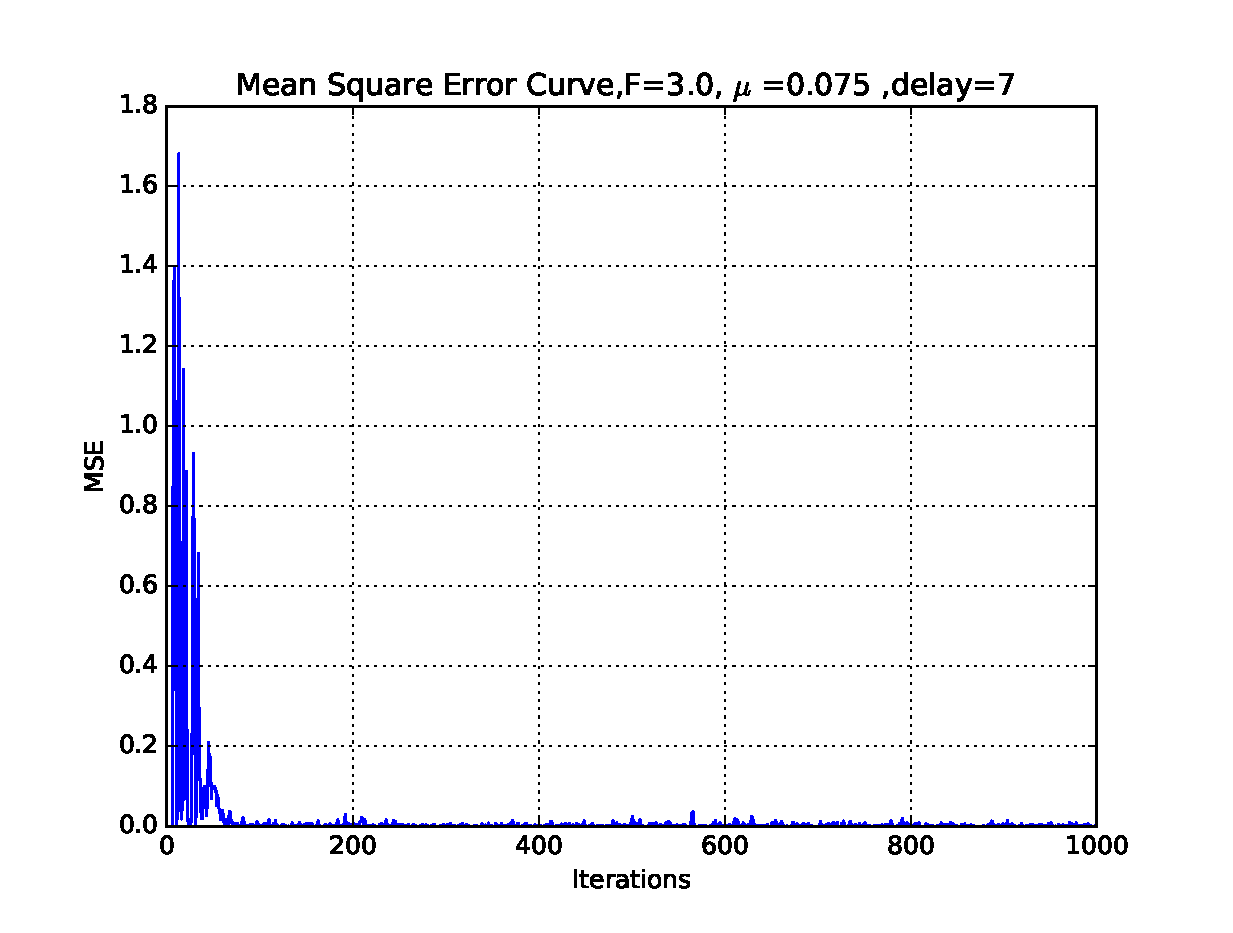
\includegraphics[width=\columnwidth]{Learning_curve.eps}
%\caption{}
%\label{fig:f3}
%\end{figure}
\begin{figure}[h]
	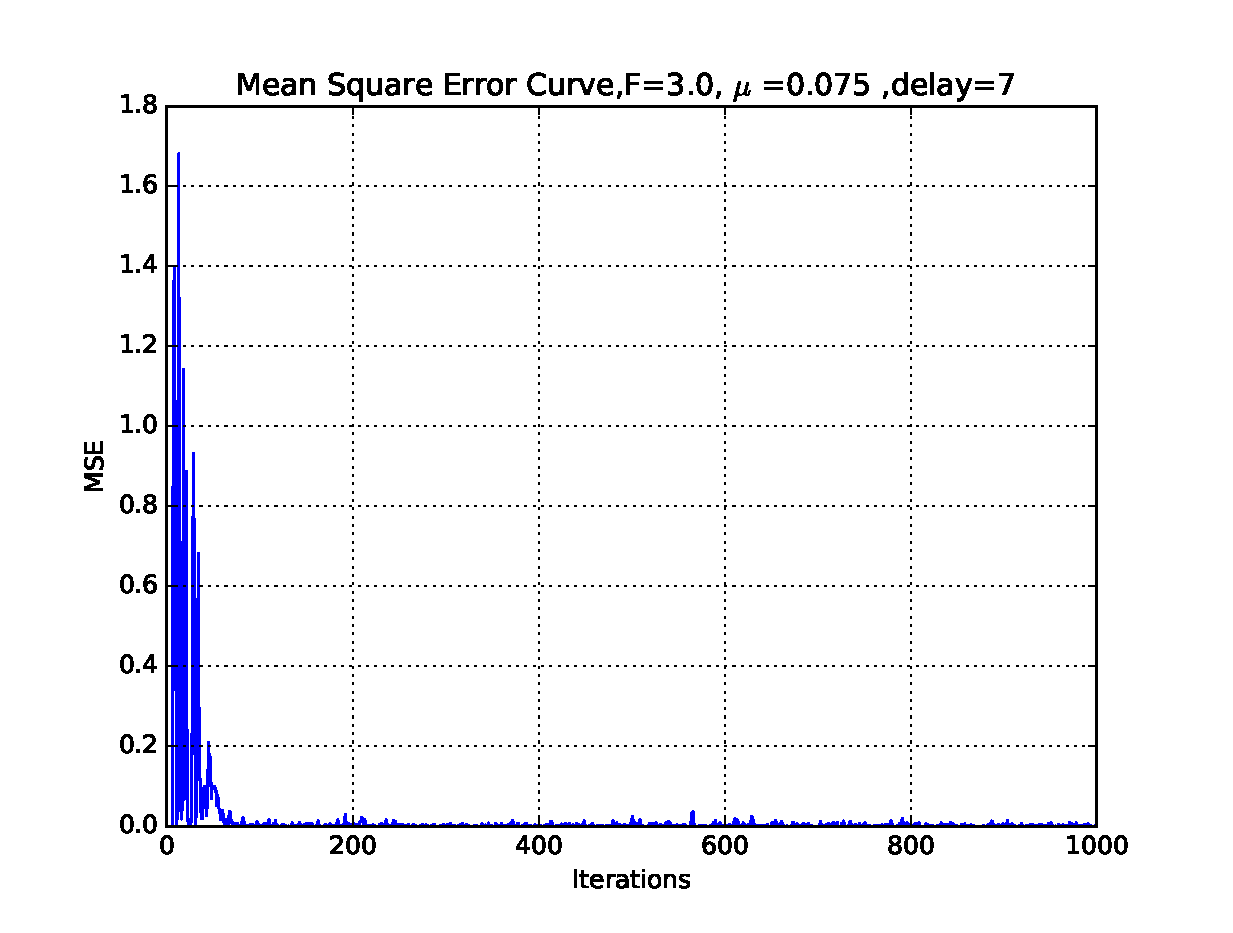
\includegraphics[width=1\linewidth]{Learning_curve.eps}
	
%	\caption{Circuit_Diagram}
	\label{}
	\caption{}
\label{fig:f3}

\end{figure}
\begin{problem}
Repeat the problem \ref{prob3.1} with different number of tap weights in the FIR LMS adaptive filter. For example you could consider 9, or 11 tap weights.Estimate the amount of delay you need based on the number of tap weights you are using. Comment.\label{prob3.2}
\end{problem}
\begin{problem}
Repeat the problem \ref{prob3.1} with different $\mu$=0.025,0.05,0.0075. What do you observe? \label{prob3.3}
\end{problem}

\begin{problem}
Repeat the problem \ref{prob3.1} with different variance for AWGN. What do you observe? \label{prob3.3}
\end{problem}
\begin{problem}
At the output of the adaptive filter have a hard threshold unit to classify the output as 1 or -1. This is done since we know that the transmitted symbols were 1 or -1. Now write a python script to compute the percentage bits that are in error at convergence (this will give you the bit error rate (BER)) with different SNRs. Plot the SNR Vs BER curve.
\end{problem}
\solution
	  \lstinputlisting{./LMS_BER.py}
\begin{center}
\begin{figure}
\centering
\includegraphics[width=\columnwidth]{SNR_Vs_BER.eps}
\caption{}
\label{fig:f3}
\end{figure}
\end{center}

\begin{problem}

The channel is no longer as given by the cosine function. But, now let the channel be modeled by an FIR filter of length 10, and each FIR coefficient be of unit magnitude. Repeat the above channel equalization problem for the equalizer under a narrow band channel.Plot the bit error rate.
\end{problem}
\begin{problem}
The data symbols are not binary (BPSK) but are QPSK. You can generalize the method used for generating BPSK to a method for generating QPSK. Plot the bit error rate. Do this for both the cases: (a) the FIR channel specified above, and (b) any other narrow band channel of your choice.
\end{problem}

\end{document}